\documentclass[border=3pt]{standalone}
\usepackage[sfdefault]{FiraSans}
\usepackage{amsmath,amssymb}
\usepackage{tikz}
\usetikzlibrary{arrows.meta,shapes.geometric,shapes.misc,shadows,calc,positioning,decorations.pathmorphing}

% ---------------- palette ----------------
\definecolor{inkA}{HTML}{2F4B7C}   \definecolor{bgA}{HTML}{EEF3FA}   \definecolor{lnA}{HTML}{A9BEDC}
\definecolor{inkB}{HTML}{5B3F8C}   \definecolor{bgB}{HTML}{F3EFFA}   \definecolor{lnB}{HTML}{BFAEDC}
\definecolor{inkC}{HTML}{1F6E54}   \definecolor{bgC}{HTML}{EDF7F1}   \definecolor{lnC}{HTML}{9CCDB2}
\definecolor{caro}{HTML}{F7D6DA}   \definecolor{caroL}{HTML}{D9828E}
\definecolor{mela}{HTML}{D7E8F7}   \definecolor{melaL}{HTML}{7FA8D1}
\definecolor{heat1}{HTML}{FDE7CF}  \definecolor{heat2}{HTML}{F9B86B}  \definecolor{heat3}{HTML}{E8762B}
\definecolor{cold}{HTML}{FFFFFF}   \definecolor{grayL}{HTML}{8A8F98}  \definecolor{okG}{HTML}{2A9D73}
\definecolor{plane3}{HTML}{E9E1F6} \definecolor{plane2}{HTML}{E4E9F7} \definecolor{plane1}{HTML}{E2F1EC} \definecolor{plane0}{HTML}{F6EEE3}

\tikzset{
  panel/.style={rounded corners=10pt, line width=0.6pt},
  ptitle/.style={font=\bfseries\small, anchor=west},
  soft/.style={rounded corners=6pt, line width=0.55pt, drop shadow={opacity=0.12, shadow xshift=0.6pt, shadow yshift=-0.8pt}},
  bubble/.style={soft, align=left, font=\tiny, inner sep=3.5pt, text width=36mm,
                 execute at begin node={\hyphenpenalty=10000\exhyphenpenalty=10000}},
  tag/.style={rounded corners=2.5pt, font=\tiny\ttfamily, inner sep=1.6pt, fill=white, draw=grayL!70},
  flow/.style={-{Stealth[length=2.4mm, width=2mm, round]}, line width=0.9pt, line cap=round},
  thin/.style={line width=0.45pt},
  cap/.style={font=\tiny, text=grayL, align=center},
  node0/.style={circle, minimum size=2.1mm, inner sep=0pt, draw=grayL, line width=0.4pt},
}

% ---------------- icons ----------------
\tikzset{
  pics/person/.style n args={2}{code={
    \fill[#1] (0,0.16) circle (0.12);
    \fill[#1] (-0.2,-0.2) .. controls (-0.2,0.03) and (0.2,0.03) .. (0.2,-0.2) -- cycle;
    \node[font=\tiny\bfseries, text=white] at (0,0.16) {#2};
  }},
  pics/lock/.style={code={
    \draw[line width=0.7pt, grayL!90!black] (-0.07,0.02) -- (-0.07,0.09) arc (180:0:0.07) -- (0.07,0.02);
    \fill[grayL!90!black, rounded corners=0.6pt] (-0.11,-0.12) rectangle (0.11,0.04);
    \fill[white] (0,-0.04) circle (0.018);
  }},
  pics/shield/.style={code={
    \fill[#1] (0,0.24) .. controls (0.12,0.2) and (0.2,0.2) .. (0.22,0.18) -- (0.22,0.02)
      .. controls (0.22,-0.14) and (0.1,-0.22) .. (0,-0.27) .. controls (-0.1,-0.22) and (-0.22,-0.14) .. (-0.22,0.02)
      -- (-0.22,0.18) .. controls (-0.2,0.2) and (-0.12,0.2) .. (0,0.24) -- cycle;
    \draw[white, line width=1.1pt, line cap=round, line join=round] (-0.09,-0.01) -- (-0.02,-0.08) -- (0.1,0.07);
  }},
  pics/magnifier/.style={code={
    \draw[#1, line width=1.3pt] (0,0) circle (0.13);
    \draw[#1, line width=1.8pt, line cap=round] (0.1,-0.1) -- (0.24,-0.24);
  }},
  pics/chip/.style 2 args={code={
    \foreach \i in {-0.14,0,0.14} {
      \draw[#1, line width=0.8pt] (\i,0.26) -- (\i,0.33); \draw[#1, line width=0.8pt] (\i,-0.26) -- (\i,-0.33);
      \draw[#1, line width=0.8pt] (0.26,\i) -- (0.33,\i); \draw[#1, line width=0.8pt] (-0.26,\i) -- (-0.33,\i); }
    \fill[#1, rounded corners=2.5pt] (-0.26,-0.26) rectangle (0.26,0.26);
    \node[font=\tiny\bfseries, text=white] at (0,0) {#2};
  }},
  pics/calendar/.style={code={
    \draw[grayL, line width=0.5pt, rounded corners=0.8pt] (-0.09,-0.08) rectangle (0.09,0.08);
    \fill[grayL] (-0.09,0.04) rectangle (0.09,0.08);
  }},
}

\begin{document}
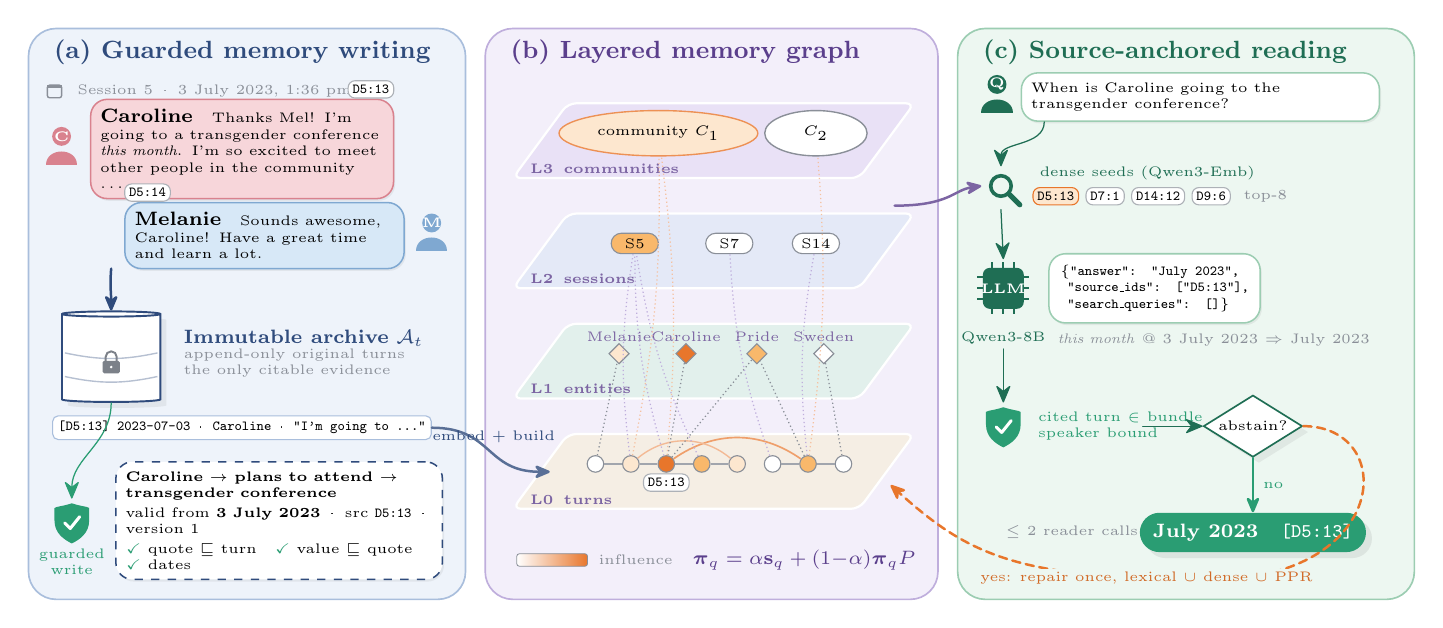
\begin{tikzpicture}[x=1cm, y=1cm]

% ======================= panels =======================
\draw[panel, fill=bgA, draw=lnA] (0,0) rectangle (5.55,7.25);
\draw[panel, fill=bgB, draw=lnB] (5.8,0) rectangle (11.55,7.25);
\draw[panel, fill=bgC, draw=lnC] (11.8,0) rectangle (17.6,7.25);
\node[ptitle, text=inkA] at (0.2,6.95) {(a) Guarded memory writing};
\node[ptitle, text=inkB] at (6.0,6.95) {(b) Layered memory graph};
\node[ptitle, text=inkC] at (12.0,6.95) {(c) Source-anchored reading};

% ======================= (a) writing =======================
\pic at (0.33,6.45) {calendar};
\node[font=\tiny, text=grayL, anchor=west] at (0.5,6.45) {Session 5 \,·\, 3 July 2023, 1:36 pm};
\pic at (0.42,5.72) {person={caroL}{C}};
\node[bubble, fill=caro, draw=caroL, anchor=west] (b1) at (0.78,5.72)
  {\textbf{\scriptsize Caroline}\quad Thanks Mel! I'm going to a transgender conference \emph{this month}. I'm so excited to meet other people in the community \dots};
\node[tag, anchor=south east] at (b1.north east) {D5:13};
\pic at (5.12,4.62) {person={melaL}{M}};
\node[bubble, fill=mela, draw=melaL, anchor=east, text width=33mm] (b2) at (4.78,4.62)
  {\textbf{\scriptsize Melanie}\quad Sounds awesome, Caroline! Have a great time and learn a lot.};
\node[tag, anchor=south west] at (b2.north west) {D5:14};

% archive cylinder
\node[cylinder, shape border rotate=90, aspect=0.28, minimum width=1.25cm, minimum height=1.15cm,
      draw=inkA, fill=white, line width=0.7pt, drop shadow={opacity=0.12}] (arch) at (1.05,3.05) {};
\draw[inkA!35, line width=0.5pt] ($(arch.west)+(0.05,0.08)$) to[bend right=12] ($(arch.east)+(-0.05,0.08)$);
\draw[inkA!35, line width=0.5pt] ($(arch.west)+(0.05,-0.22)$) to[bend right=12] ($(arch.east)+(-0.05,-0.22)$);
\pic at ($(arch.center)+(0,-0.06)$) {lock};
\node[anchor=west, align=left, font=\scriptsize, text=inkA] at (1.85,3.32) {\textbf{Immutable archive} $\mathcal{A}_t$};
\node[anchor=west, align=left, font=\tiny, text=grayL] at (1.85,3.0) {append-only original turns\\the only citable evidence};
\node[anchor=west, font=\tiny\ttfamily, fill=white, rounded corners=2pt, draw=lnA, inner sep=2pt] (rec) at (0.3,2.18)
  {[D5:13] 2023-07-03 · Caroline · "I'm going to ..."};
\draw[flow, inkA] (1.05,4.2) to[out=-95, in=90] (arch.north);

% guarded write -> versioned note
\pic at (0.55,0.98) {shield=okG};
\node[font=\tiny, text=okG, align=center] at (0.55,0.48) {guarded\\write};
\node[soft, draw=inkA, dashed, fill=white, align=left, anchor=west, inner sep=3.5pt, font=\tiny, text width=39mm] (note) at (1.1,1.0)
  {\textbf{Caroline} $\rightarrow$ \textbf{plans to attend} $\rightarrow$ \textbf{transgender conference}\\[1pt]
   valid from \textbf{3 July 2023} \,·\, src \texttt{D5:13} \,·\, version 1\\[1pt]
   {\color{okG}\checkmark} quote $\sqsubseteq$ turn \; {\color{okG}\checkmark} value $\sqsubseteq$ quote \; {\color{okG}\checkmark} dates};
\draw[flow, okG, thin] (arch.south) to[out=-90, in=90] (0.55,1.28);

% ======================= (b) layered graph =======================
% planes: (x0, y) bottom-left, width 4.4, skew 0.7, height 0.95
\foreach \y/\c/\lab in {5.35/plane3/L3\enspace communities, 3.95/plane2/L2\enspace sessions, 2.55/plane1/L1\enspace entities, 1.15/plane0/L0\enspace turns} {
  \fill[\c, opacity=0.95, rounded corners=3pt] (6.15,\y) -- (10.55,\y) -- (11.25,\y+0.95) -- (6.85,\y+0.95) -- cycle;
  \draw[white, line width=0.8pt, rounded corners=3pt] (6.15,\y) -- (10.55,\y) -- (11.25,\y+0.95) -- (6.85,\y+0.95) -- cycle;
  \node[font=\tiny\bfseries, text=inkB!80, anchor=west] at (6.25,\y+0.12) {\lab};
}
% L0 turns (heat = PPR influence)
\foreach \x/\h/\n in {7.2/cold/a,7.65/heat1/b,8.1/heat3/s,8.55/heat2/c,9.0/heat1/d,9.45/cold/e,9.9/heat2/f,10.35/cold/g} {
  \node[node0, fill=\h] (t\n) at (\x,1.72) {};
}
\draw[grayL!80, thin] (ta) -- (tb) -- (ts) -- (tc) -- (td);  \draw[grayL!80, thin] (te) -- (tf) -- (tg);
\draw[heat3!70, line width=0.6pt] (ts) to[bend left=35] (tf);
\draw[heat3!50, line width=0.5pt] (tb) to[bend left=40] (td);
\node[tag, anchor=north] at ($(ts)+(0,-0.12)$) {D5:13};
% L1 entities (capitalized tokens, as extracted)
\foreach \x/\h/\n/\l in {7.5/heat1/m/Melanie, 8.35/heat3/g/Caroline, 9.25/heat2/c/Pride, 10.1/cold/s/Sweden} {
  \node[diamond, minimum size=2.6mm, inner sep=0pt, draw=grayL, fill=\h, line width=0.4pt] (e\n) at (\x,3.12) {};
  \node[font=\tiny, text=inkB!80] at ($(e\n)+(0,0.22)$) {\l};
}
% L2 sessions
\foreach \x/\h/\n/\l in {7.7/heat2/1/S5, 8.9/cold/2/S7, 10.0/cold/3/S14} {
  \node[rounded rectangle, minimum width=6mm, minimum height=2.6mm, inner sep=0pt, draw=grayL, fill=\h, line width=0.4pt,
        font=\tiny] (s\n) at (\x,4.52) {\l};
}
% L3 communities
\node[ellipse, minimum width=15mm, minimum height=4.5mm, draw=heat3!80, fill=heat1, line width=0.5pt, font=\tiny] (c1) at (8.0,5.92) {community $C_1$};
\node[ellipse, minimum width=13mm, minimum height=4.5mm, draw=grayL, fill=white, line width=0.5pt, font=\tiny] (c2) at (10.0,5.92) {$C_2$};
% inter-layer links
\foreach \a/\b in {ts/eg, ts/ec, tf/ec, ta/em, tg/es} \draw[grayL, densely dotted, thin] (\a) -- (\b);
\foreach \a/\b in {ts/s1, tb/s1, tc/s1, te/s2, tf/s3} \draw[lnB, densely dotted, thin] (\a) to[bend left=8] (\b);
% communities are Louvain clusters of turns: member edges go to L0 turns
\foreach \a/\b in {ts/c1, tb/c1, tf/c2} \draw[heat3!45, densely dotted, thin] (\a) to[bend right=6] (\b);
% PPR legend + formula
\shade[left color=cold, right color=heat3, draw=grayL, line width=0.3pt, rounded corners=1pt] (6.2,0.42) rectangle (7.1,0.58);
\node[font=\tiny, text=grayL, anchor=west] at (7.12,0.5) {influence};
\node[font=\scriptsize, text=inkB] at (9.85,0.5) {$\boldsymbol\pi_q=\alpha\mathbf{s}_q+(1{-}\alpha)\boldsymbol\pi_q P$};

% cross-panel: archive -> graph
\draw[flow, inkA!80] (rec.east) .. controls (5.9,2.18) and (5.8,1.62) .. node[pos=0.55, above, font=\tiny, text=inkA] {embed + build} (6.62,1.62);

% ======================= (c) reading =======================
\pic at (12.3,6.38) {person={inkC}{Q}};
\node[bubble, fill=white, draw=lnC, anchor=west, text width=43mm] (qq) at (12.6,6.38)
  {When is Caroline going to the transgender conference?};

% step 1: seeds
\pic at (12.35,5.25) {magnifier=inkC};
\node[font=\tiny, text=inkC, anchor=west] at (12.72,5.42) {dense seeds (Qwen3-Emb)};
\node[tag, draw=heat3, fill=heat1, anchor=west] (k1) at (12.75,5.12) {D5:13};
\node[tag, anchor=west] (k2) at ($(k1.east)+(0.08,0)$) {D7:1};
\node[tag, anchor=west] (k3) at ($(k2.east)+(0.08,0)$) {D14:12};
\node[tag, anchor=west] (k4) at ($(k3.east)+(0.08,0)$) {D9:6};
\node[font=\tiny, text=grayL, anchor=west] at ($(k4.east)+(0.04,0)$) {top-8};
\draw[flow, inkC, thin] (qq.south west) ++(0.3,0) to[out=-90, in=90] (12.35,5.5);

% step 2: reader
\pic at (12.38,3.95) {chip={inkC}{LLM}};
\node[font=\tiny, text=inkC, anchor=north] at (12.38,3.52) {Qwen3-8B};
\node[soft, draw=lnC, fill=white, anchor=west, align=left, font=\tiny\ttfamily, inner sep=4pt] (json) at (12.95,3.95)
  {\{"answer": "July 2023",\\ \ "source\_ids": ["D5:13"],\\ \ "search\_queries": []\}};
\node[font=\tiny, text=grayL, anchor=north west, align=left] at (json.south west) {\emph{this month} @ 3 July 2023 $\Rightarrow$ July 2023};
\draw[flow, inkC, thin] (12.35,4.95) -- (12.38,4.32);

% step 3: checks + gate
\pic at (12.38,2.2) {shield=okG};
\node[font=\tiny, text=okG, anchor=west, align=left] at (12.7,2.2) {cited turn $\in$ bundle\\speaker bound};
\node[diamond, aspect=1.6, draw=inkC, fill=white, line width=0.6pt, font=\tiny, inner sep=1pt, drop shadow={opacity=0.12}] (gate) at (15.55,2.2) {abstain?};
\draw[flow, inkC, thin] (12.38,3.18) -- (12.38,2.5);
\draw[flow, inkC, thin] (14.15,2.2) -- (gate.west);

% answer
\node[rounded rectangle, fill=okG, text=white, font=\scriptsize\bfseries, inner sep=4pt, drop shadow={opacity=0.15}] (ans) at (15.55,0.85)
  {July 2023 \;\;\textmd{\texttt{[D5:13]}}};
\draw[flow, okG] (gate.south) -- node[right, font=\tiny, text=okG] {no} (ans.north);
\node[font=\tiny, text=grayL] at (13.25,0.85) {$\le$ 2 reader calls};

% repair loop back to the graph
\draw[flow, heat3, line width=0.9pt, dash pattern=on 3pt off 2pt]
  (gate.east) .. controls (17.4,2.2) and (17.3,0.25) .. (15.0,0.25)
  .. controls (12.5,0.25) and (11.9,0.6) .. (10.95,1.45);
\node[font=\tiny, text=heat3!90!black, fill=bgC, inner sep=1pt] at (14.2,0.27) {yes: repair once, lexical $\cup$ dense $\cup$ PPR};

% cross-panel: graph -> reading (seeds / influence)
\draw[flow, inkB!80] (11.0,5.0) .. controls (11.7,5.0) and (11.75,5.2) .. (12.1,5.25);

\end{tikzpicture}
\end{document}
